\section{Open Question} \label{rotation}

\subsection{Overview}
This section considers an open question: how to enhance the robustness of distributed embedded control systems utilizing the weakly hard model. The solution of this question can be applied to improving the security and robustness of automatic vehicles. A classical method to enhance the robustness of distributed system is to increase the redundancy of the system components so that single-point failure can be avoided. However, embedded control systems, e.g. control systems on automatic vehicles, have limited resources and therefore cannot afford a high level of redundancy. On the other hand, control systems can tolerant a certain level of occasional, bounded deadline misses as demonstrated in~\cite{liang2019security, maggio2020control, ramanathan1999overload, goswami2014relax, horssen2016performance, linsenmayer2017stabilization, pazzaglia2018beyond}. Therefore, we can utilize this property to optimize the assignments of application-level control tasks on processors. 

The approach is as follows: first, we analyze the deadline miss pattern for each control task in the m-K weakly hard model (Definition~\ref{def:missany}). Then, we map the control tasks to processors in a way that the tasks are rotating to a different processor in the next time stamp. Each time a processor encounters fatal errors and stops working, we adjust the mapping to fulfill the stability and control performance requirements for each control task, based on its deadline miss pattern. The mapping problem can be formulated as a MIP problem that optimizes the stability and control performance of the task set. Figure~\ref{fig:rotationmap} presents a model of two control tasks that are mapped onto two processor cores. 

\begin{figure}[h]
\caption{A model of systems with rotational control tasks mapping}
\centering
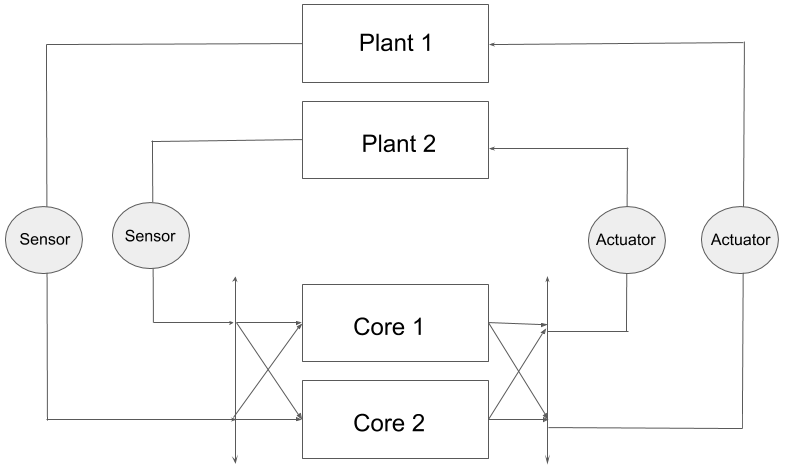
\includegraphics[width=0.5\textwidth]{rotationmap}
\label{fig:rotationmap}
\end{figure}

\subsection{Deadline Miss Pattern}
We consider the deadline miss pattern for each control task in the m-K weakly hard model (Definition~\ref{def:missany}). We assume that the system platform adopts a static-priority based, preemptive policy. A task set is defined as follows:
\begin{align*}
\tau = \{\tau_1, \tau_2, ..., \tau_n\}
\end{align*}
$\forall i \in {1, 2, ..., n}$, $\tau_i$ is a tuple of the following form:
\begin{align*}
\tau_i  = (c_{\tau_i}, d_{\tau_i}, t_{\tau_i}, p_{\tau_i})
\end{align*}
where $c_{\tau_i}$ is the worst-case execution time (WECT), $d_{\tau_i}$ is the deadline, $t_{\tau_i}$ is the period, and $p_{\tau_i}$ is the priority of $\tau_i$. 

We can use analysis technique proposed in~\cite{liang2019security, goswami2014relax} to analytically calculate an upper bound on the deadline miss pattern for each control task that ensures the stability of the task. 

\subsection{Objective Function}
We formulate the control tasks mapping problem as an MIP problem. The objective of this MIP formulation is to optimize the stability and control performance of the control tasks. To optimize the stability, we define a variable \textit{S} such that 
\begin{align*}
S &= \sum_{i=1}^n b_i \\
b_i &= \twopartdef {0} {\tau_i \: is \: stable} {1} {\tau_i \: is \: unstable}
\end{align*}
Here, \textit{$b_i$} is a binary decision variable that represents whether task $\tau_i$ is table or not. Then, by minimizing \textit{S}, we can have the maximum number of tasks that fulfill the stability requirement.

For control performance requirement, we can use the method described in Section ~\ref{stability and control performance}, as well as in ~\cite{liang2019security}, to describe the number of minimum required sample intervals needed to bring the system which is suffered from a disturbance back to the equilibrium state. We use \textit{H} to describe the control performance for all tasks. Thus, the objective function is:
\begin{align*}
minimize \;&\alpha\textit{S} + \beta\textit{H}
\end{align*}
where $\alpha$ and $\beta$ are predefined weights that are used to study the trade-off between two objectives.

\subsection{Constraints}
We now attempt to create constraints for the MIP formulation. The first type of constraints ensures that control tasks and communication tasks are collision-free, so that at any given time stamp, at most one control task will be running on any processor core, and at most one communication task will be transmitted on any communication bus. The formulation of a similar type of constraint is proposed in~\cite{Zhang2018SynthesizingCA}.

We then formulate constraints that encode the data dependency requirement for control tasks as well as path dependency requirement for communication tasks. Data dependency ensures that control tasks and their corresponding communication tasks are executed in the correct temporal order. Path dependency similarly impose temporal order to communication tasks so that they can be transmitted to the correct destination. Zhang ~\cite{Zhang2018SynthesizingCA} provides a general type of dependency constraint that can be of use in this solution.

Next, we encode timing constraints for the response time and end-to-end latency of each task. We use the method introduced in Section~\ref{weakly hard constraints formulation}~\cite{liang2019security} to set weakly hard constraints on tasks, and for those tasks not schedulable on the weakly hard model, hard constraints with a predefined maximum time requirement can be used.

Constraints are needed to ensure that the control tasks mapping will be changed from a time stamp to the next one. If we run the mapping algorithm every time stamp, so on each time stamp, we can encode the current mapping to be different from a predefined constant N which represents the number of past mappings in the most recent time stamps. However, the time to run the mapping algorithm on each time stamp is expensive in terms of time, and we will need to take this delay into our consideration. We can use heuristic search algorithm to aid the solving process of the MIP problem. An alternative approach is to analytically solve the MIP problem once with a default mapping to be in a round-robin manner. We predefine a temporal order of processor cores that each task by default is mapped to for each round. In this way, we don't need to run the MIP problem in run time and we do not need to have constraints about the order of processors each task is mapping to at every time stamp.

















